\chapter{Cross-loop Optimization of Arithmetic Intensity for Finite Element Integration}
\label{ch:lowlevelopt}

In the previous chapter, a method to minimize the operation count of finite element integration loop nests, or ``assembly kernels'', has been developed. The focus is now on the same class of kernels, but a complementary issue is tackled: the low level optimization of the generated code. 

\section{Recapitulation and Objectives}

We know that an assembly kernel is characterized by the presence of an affine, often non-perfect loop nest, in which individual loops are rather small: their trip count rarely exceeds 30, and may be as low as 3 for low order methods. In the innermost loop, a compute intensive expression evaluates an $n$-dimensional array, or element tensor, which represents the result of local assembly in an element of the discretized domain. More specifically: in bilinear forms, $n=2$ and the output is referred to as element matrix; in linear forms, $n=1$ and the output is referred to as element vector. With such a kernel structure, the objective of the low level optimization is maximizing register locality and SIMD vectorization.

We aim to maximize our impact on the platforms that are realistically used for finite element applications, so we target conventional CPU architectures rather than GPUs. The key limiting factor to the execution on GPUs is the stringent memory requirements. Only relatively small problems fit in a GPU memory, and support for distributed GPU execution in general purpose finite element frameworks is minimal. There has been some research on adapting local assembly to GPUs, although it differs from ours in several ways, including: (i) not relying on automated code generation from a domain-specific language, (ii) testing only very low order methods, (iii) not optimizing for cross-loop arithmetic intensity (the goal is rather effective multi-thread parallelization). In addition, our code transformations would drastically impact the GPU parallelization strategy, for example by increasing a thread's working set. For all these reasons, a study on extending the research to GPU architectures is beyond the scope of this work. The related work on the subject is covered in Section~\ref{sec:coffee-related-work}, while intuitions about this research direction are provided in Section~\ref{sec:generality}.

Achieving high-performance on CPUs is non-trivial. The complexity of the mathematical expressions, which we know to be often characterized by a large number of operations on constants and small vectors, makes it hard to determine a single or specific sequence of transformations that is successfully applicable to all problems. Loop trip counts are typically small and can vary significantly, which further exacerbates the issue. Moreover, the memory access pattern can be either unit-stride (\texttt{A[i]}, \texttt{A[i+1]}, \texttt{A[i+2]}, ...) or multi-stride (\texttt{A[i]}, \texttt{A[i+1]}, \texttt{A[i+N]}, \texttt{A[i+N+1]}, ...) -- for example, as a consequence of skipping useless floating-point operations, see Section~\ref{sec:zeros}. We will show that general-purpose compilers, such as \emph{GNU's} and \emph{Intel's}, fail at maximizing the efficiency of the generated code because of such a particular structure. Polyhedral-model-based source-to-source compilers, for instance~\cite{pluto}, can apply aggressive loop optimizations, such as tiling, but these are not particularly helpful in our context since they mostly focus on cache locality. 

As in Chapter~\ref{ch:optimality}, we focus on optimizing the performance of assembly kernels produced through automated code generation, so we seek transformations that are generally applicable and effective. In particular, we introduce and study the following transformations:

\begin{description}
\item[Padding and data alignment] SIMD vectorization is more effective when the CPU registers are packed (unpacked) by means of aligned load (store) instructions. Data alignment is achieved through array padding, a conceptually simple yet powerful transformation that can result in dramatic reductions in execution time. 
\item[Vector-register tiling] Tiling at the level of vector registers exploits the peculiar memory access pattern induced by finite element operators (i.e., the linearity of the test and trial functions loops) to improve data locality.
\item[Expression splitting] Complex expressions are often characterized by high register pressure (i.e., the lack of available registers inducing the compiler to ``spill'' data from registers to cache). This transformation exploits the associativity property of the addition to distribute, or ``split'', an expression into multiple sub-expressions to be computed in separate loop nests.
\end{description}
Further, we analyze the effects of ``more traditional'' optimizations: loop unroll, loop interchange, loop fusion and vector promotion. Some of these are not applied by general-purpose compilers, or are applied in a sub-optimal way; in such a case, they are introduced explicitly through our compiler, COFFEE. 

To summarize, the contributions of this chapter are:
\begin{itemize}
\item The introduction of novel transformations for optimizing the performance of assembly kernels. Some of these transformations exploit properties of assembly kernels.
\item An extensive analysis of common compiler transformations, specialized to take advantage of the structure of assembly kernels.
\item Extensive experimentation using a set of real-world forms commonly arising in finite element methods.
\item A discussion concerning the generality of the transformations and their applicability to different domains.
\end{itemize}

\section{Low-level Optimization}
\label{sec:lowlevelopt}


\subsection{Padding and Data Alignment}
\label{sec:coffee-padding}
The absence of stencils renders the local element matrix computation easily auto-vectorizable by a general-purpose compiler\footnote{In practice, however, open source compilers such as {\em GCC} and {\em LLVM} reject auto-vectorization if the loops are too small. This denotes serious issues in their cost models.}. Nevertheless, auto-vectorization is not efficient if data are not aligned to cache-line boundaries and if the length of the innermost loop is not a multiple of the vector length $\mbox{\texttt{VL}}$, especially when the loops are small as in local assembly. 

Data alignment is enforced in two steps. Firstly, all arrays (but the element matrix, for reasons discussed shortly) are padded by rounding the innermost dimension to the nearest multiple of $\mbox{\texttt{VL}}$. For instance, assume the original size of a basis function array is 3$\times$3 and $\mbox{\texttt{VL}}=4$ (e.g. AVX processor, with 32-byte long vector registers and 8-byte double-precision floats). In this case, a padded version of the array will have size 3$\times$4. Secondly, their base address is enforced to multiples of $\mbox{\texttt{VL}}$ by means of special attributes. The compiler is explicitly told about data alignment using suitable pragmas. For example, in the case of the Intel compiler, the annotation \texttt{$\#$pragma vector aligned} is added before a loop (as shown in later figures) to inform that all of the memory accesses in the loop body will be aligned. This allows the compiler to issue aligned load and store instructions, which are significantly faster than unaligned ones.

In our computational model, the element matrix is one of the kernel's input parameters, so it needs special handling when padding (the signature of the kernel must not be changed, otherwise the abstraction would be broken). We create a ``shadow'' copy of the element matrix, padded, aligned, and initialized to 0. The shadow element matrix is used in place of the original element matrix. Right before returning to the caller, a loop nest copies, discarding the padded region, the shadow matrix back into the input buffer.

Array padding also allows to safely round the loop trip count to the nearest multiple of $\mbox{\texttt{VL}}$. This avoids the introduction of a remainder (scalar) loop from the compiler, which would render vectorization less efficient. These extra iterations only write to the padded region of the element matrix, and therefore have no side effects on the final result.

Listing~\ref{code:weighted-laplace-licm-pad} illustrates the effect of padding and data alignment on top of generalized code motion applied to the weighted Laplace operator which we introduced in Chapter~\ref{ch:background}.

\setcounter{algocf}{0}% Modify counter of algorithm
\begin{algorithm}
\scriptsize\ttfamily
\SetAlgorithmName{LISTING}{}

\KwSty{void} weighted$\_$laplace(\KwSty{double} A[3][3], \KwSty{double} **coords, \KwSty{double} w[3]) $\lbrace$\\
~~\KwSty{$\#$define} ALIGN $\_\_$attribute$\_\_$((aligned(32))) \\
~~// K, det = Compute Jacobian (coords) \\
~~\\
~~// Quadrature weights \\
~~\KwSty{static const double} W[6] ALIGN = {0.5}; \\
~~\\
~~// Basis functions \\
~~\KwSty{static const double} B[6][4] ALIGN = $\lbrace\lbrace$...$\rbrace\rbrace$ ;\\
~~\KwSty{static const double} C[6][3] ALIGN = $\lbrace\lbrace$...$\rbrace\rbrace$ ;\\
~~\KwSty{static const double} D[6][4] ALIGN = $\lbrace\lbrace$...$\rbrace\rbrace$ ;\\
~~\\
~~// Padded buffer \\
~~\KwSty{double} PA[3][4] ALIGN = $\lbrace\lbrace$0.0$\rbrace\rbrace$;\\
~~\\
~~\KwSty{for} (\KwSty{int} i = 0; i$<$6; i++) $\lbrace$ \\
~~~~\KwSty{double} f0  = 0.0;\\
~~~~\KwSty{for} (\KwSty{int} r  = 0; r < 3; ++r) $\lbrace$ \\
~~~~~~f0 += (w[r] * C[i][r]);\\
~~~~$\rbrace$ \\
~~~~\KwSty{double} T0[4] ALIGN;\\
~~~~\KwSty{double} T1[4] ALIGN;\\
~~~~\KwSty{$\#$pragma vector aligned}\\
~~~~\KwSty{for} (\KwSty{int} k = 0; k$<$4; r++) $\lbrace$ \\
~~~~~~T0[k] = ((K[1]*B[i][k])+(K[3]*D[i][k]));\\
~~~~~~T1[k] = ((K[0]*B[i][k])+(K[2]*D[i][k]));\\
~~~~$\rbrace$\\
~~~~\KwSty{for} (\KwSty{int} j = 0; j$<$3; j++) $\lbrace$\\
~~~~~~\KwSty{$\#$pragma vector aligned}\\
~~~~~~\KwSty{for} (\KwSty{int} k = 0; k$<$4; k++) $\lbrace$\\
~~~~~~~~PA[j][k] += (T0[k]*T0[j] + T1[k]*T1[j])*det*W[i]*f0);\\
~~~~~~$\rbrace$\\
~~~~$\rbrace$\\
~~$\rbrace$\\
$\rbrace$\\
\KwSty{for} (\KwSty{int} j = 0; j$<$3; j++) $\lbrace$\\
~~\KwSty{for} (\KwSty{int} k = 0; k$<$3; k++) $\lbrace$\\
~~~~A[j][k] = PA[j][k];\\
~~$\rbrace$\\
$\rbrace$\\

\caption{The assembly kernel for the weighted Laplace operator in Listing~\ref{code:weighted-laplace} after application of padding and data alignment (on top of generalized code motion). An AVX architecture, which implies $\mbox{\texttt{VL}}=4$, is assumed.}
\label{code:weighted-laplace-licm-pad}
\end{algorithm}

%\subsubsection{Example}
%Consider again the code in Figure~\ref{fig:withzeros-skipped-code} and assume $\mbox{\texttt{VL}}=4$ double-precision floats (i.e. vector registers are 32 bytes longs). 
%
%The arrays in the loop nest \texttt{[j1,k1]} can be padded and the right bound of loop \texttt{k1} can be safely increased to 8: eventually, values computed in the region \texttt{M[0:3][6:8]} will be discarded. Then, by explicitly aligning arrays using suitable qualifiers (e.g. \texttt{$\#\_\_$attribute$\_\_$((aligned(32)))} for the Intel compiler), effective SIMD auto-vectorization can be obtained for this loop nest. 
%
%There are some complications in the case of loops \texttt{[j0,k0]}. Here, increasing the innermost loop bound to 4 is still safe assuming that both \texttt{T1} and \texttt{A} are padded, but it has no effect: the starting addresses of the load instructions would be \texttt{$\&$T1[3]} and \texttt{$\&$A[i][3]}, which are clearly not aligned. Changing the starting address of \texttt{A} and \texttt{T1} is, in general, not an option, because these arrays could be accesses also in other loop nests, as happens with \texttt{A} in this example. One solution, instead, is to start iterating from the closest index that would ensure data alignment; in this case, $k0=0$. However, this would imply losing the effect of the zero-avoidance transformation (partially in general, totally for this loop nest). Another possibility is to attain to non-aligned accesses. Which of the two strategies is better cannot be established a-priori. An autotuning system, as described in Section~\ref{sec:coffee-autotune}, will help answering this question.
%
%Finally, note that whenever increasing a loop bound cause accessing non-zero entries in the local element matrix \texttt{M}, there is no way of recovering data alignment.

\subsection{Expression Splitting}
\label{sec:coffee-split}

In complex kernels, like Burgers in Listing~\ref{code:burgers}, and on certain architectures, achieving effective register allocation can be challenging. If the number of variables independent of the innermost-loop dimension is close to or greater than the number of available CPU registers, poor register reuse is likely. This usually happens when the number of basis function arrays, temporaries introduced by either generalized code motion or pre-evaluation, and problem constants is large. For example, applying code motion to the Burgers example on a 3D mesh requires 24 temporaries for the \texttt{ijk} loop order. This can make hoisting of the invariant loads out of the \texttt{k} loop inefficient on architectures with a relatively low number of registers. One potential solution to this problem consists of suitably ``splitting'' the computation of the element matrix $A$ into multiple sub-expressions. An example of this idea is given in Listing~\ref{code:weighted-laplace-split}. The transformation can be regarded as a special case of classic loop fission, in which associativity of the sum is exploited to distribute the expression across multiple loops. To the best of our knowledge, expression splitting is not supported by available compilers.

\begin{algorithm}
\scriptsize\ttfamily
\SetAlgorithmName{LISTING}{}

\KwSty{void} weighted$\_$laplace(\KwSty{double} A[3][3], \KwSty{double} **coords, \KwSty{double} w[3]) $\lbrace$\\
~~// Omitting redundant code \\
~~...\\
~~\KwSty{for} (\KwSty{int} j = 0; j$<$3; j++) $\lbrace$\\
~~~~\KwSty{for} (\KwSty{int} k = 0; k$<$3; k++) $\lbrace$\\
~~~~~~A[j][k] += (T0[k]*T0[j])*det*W[i]*f0;\\
~~~~$\rbrace$\\
~~$\rbrace$\\
~~\KwSty{for} (\KwSty{int} j = 0; j$<$3; j++) $\lbrace$\\
~~~~\KwSty{for} (\KwSty{int} k = 0; k$<$3; k++) $\lbrace$\\
~~~~~~A[j][k] += (T1[k]*T1[j])*det*W[i]*f0;\\
~~~~$\rbrace$\\
~~$\rbrace$\\
$\rbrace$\\
...
\caption{The assembly kernel for the weighted Laplace operator in Listing~\ref{code:weighted-laplace} after application of expression splitting (on top of generalized code motion). In this example, the split factor is 2.}
\label{code:weighted-laplace-split}
\end{algorithm}

Splitting an expression (henceforth \emph{split}) has, however, several drawbacks. Firstly, it increases the number of accesses to \texttt{A} in proportion to the ``split factor'', which is the number of sub-expressions produced. Also, depending on how splitting is done, it can lead to redundant computation. For example, the number of times the product \texttt{det*W3[i]} is performed is proportional to the number of sub-expressions, as shown in the code snippet. Further, it increases loop overhead, for example through additional branch instructions. Finally, it might affect register locality: for instance, the same array could be accessed in different sub-expressions, requiring a proportional number of loads be performed; this is not the case of the running example, though. Nevertheless, the performance gain from improved register reuse can still be greater if suitable heuristics are used. Our approach consists of traversing the expression tree and recursively splitting it into multiple sub-expressions as long as the number of variables independent of the innermost loop exceeds a certain threshold. This is elaborated in the next sections, and validated against empirical search in Section~\ref{sec:perf-results-split}.

\subsection{Model-driven Vector-register Tiling}
\label{sec:coffee-opvect}

\begin{algorithm}
\scriptsize\ttfamily
\SetAlgorithmName{LISTING}{}

\KwSty{void} weighted$\_$laplace(\KwSty{double} A[3][3], \KwSty{double} **coords, \KwSty{double} w[3]) $\lbrace$\\
~~// Omitting redundant code \\
~~...\\
~~// Padded buffer (note: both rows and columns) \\
~~\KwSty{double} PA[4][4] ALIGN = $\lbrace\lbrace$0.0$\rbrace\rbrace$;\\
~~\\
~~\KwSty{for} (\KwSty{int} i = 0; i$<$3; i++) $\lbrace$ \\
~~~~// Omitting redundant code \\
~~~~// ... \\
~~~~\KwSty{for} (\KwSty{int} j = 0; j$<$4; j += 4) \\
~~~~~~\KwSty{for} (\KwSty{int} k = 0; k$<$4; k += 4) $\lbrace$\\
~~~~~~~~// Sequence of \emph{LOAD} and \emph{SET} intrinsics \\
~~~~~~~~// Compute PA[0][0], PA[1][1], PA[2][2], PA[3][3] \\
~~~~~~~~// One \KwSty{$\_$mm256$\_$permute$\_$pd} per \texttt{k}-loop \emph{LOAD}\\
~~~~~~~~// Compute PA[0][1], PA[1][0], PA[2][3], PA[3][2] \\
~~~~~~~~// One \KwSty{$\_$mm256$\_$permute2f128$\_$pd} per \texttt{k}-loop \emph{LOAD}\\
~~~~~~~~// ...\\
~~~~~~$\rbrace$\\
~~~~// Scalar remainder loop (not necessary in this example)\\
~~$\rbrace$\\
~~// Restore the storage layout\\
~~\KwSty{for} (\KwSty{int} j = 0; j$<$4; j += 4) $\lbrace$\\
~~~~\KwSty{for} (\KwSty{int} k = 0; k$<$4; k += 4) $\lbrace$\\
~~~~~~\KwSty{$\_\_$m256d} r0 = \KwSty{$\_$mm256$\_$load$\_$pd} ($\&\_$A[j+0][k]);\\
~~~~~~// \emph{LOAD} PA[j+1][k], PA[j+2][k], PA[j+3][k]\\
~~~~~~r4 = \KwSty{$\_$mm256$\_$unpackhi$\_$pd} (r1, r0);\\
~~~~~~r5 = \KwSty{$\_$mm256$\_$unpacklo$\_$pd} (r0, r1);\\
~~~~~~r6 = \KwSty{$\_$mm256$\_$unpackhi$\_$pd} (r2, r3);\\
~~~~~~r7 = \KwSty{$\_$mm256$\_$unpacklo$\_$pd} (r3, r2);\\
~~~~~~r0 = \KwSty{$\_$mm256$\_$permute2f128$\_$pd} (r5, r7, 32);\\
~~~~~~r1 = \KwSty{$\_$mm256$\_$permute2f128$\_$pd} (r4, r6, 32);\\
~~~~~~r2 = \KwSty{$\_$mm256$\_$permute2f128$\_$pd} (r7, r5, 49);\\
~~~~~~r3 = \KwSty{$\_$mm256$\_$permute2f128$\_$pd} (r6, r4, 49);\\
~~~~~~\KwSty{$\_$mm256$\_$store$\_$pd} ($\&\_$A[j+0][k], r0);\\
~~~~~~// \emph{STORE} PA[j+1][k], PA[j+2][k], PA[j+3][k]\\
~~~~$\rbrace$\\
~~$\rbrace$\\
$\rbrace$\\
...
\caption{The assembly kernel for the weighted Laplace operator in Listing~\ref{code:weighted-laplace} after application of vector-register tiling (on top of generalized code motion, padding, and data alignment). In this example, the unroll-and-jam factor is 1.}
\label{code:weighted-laplace-opvect}
\end{algorithm}

One notable problem of assembly kernels concerns register allocation and register locality. The critical situation occurs when the loop trip counts and the variables accessed are such that the vector-register pressure is high. Since the kernel's working set is expected to fit the L1 cache, it is particularly important to optimize register management. Standard optimizations, such as loop interchange, unroll, and unroll-and-jam, can be employed to deal with this problem. Tiling at the level of vector registers represents another opportunity. Based on the observation that the evaluation of the element matrix can be reduced to a summation of outer products along the \texttt{j} and \texttt{k} dimensions, a model-driven vector-register tiling strategy can be implemented. If we consider the codes in the various listings and we focus on the body of the test and trial functions loops (\texttt{j} and \texttt{k}), the computation of the element matrix is abstractly expressible as
\begin{equation*}
\scriptsize
\label{outer-product}
A_{jk} = \sum_{\substack{
  x \in B' \subseteq B \\
  y \in B'' \subseteq B}}
x_j\cdot y_k ~~~~~~ j,k = 0,...,3
\end{equation*}
where $B$ is the set of all basis functions or temporary variables accessed in the kernel, whereas $B'$ and $B''$ are generic problem-dependent subsets. Regardless of the specific input problem, by abstracting from the presence of all variables independent of both \texttt{j} and \texttt{k}, the element matrix computation is always reducible to this form. Figure~\ref{fig:vect-by-vect} illustrates how we can evaluate 16 entries ($j,k=0,...,3$) of the element matrix using just 2 vector registers, which represent a 4$\times$4 tile, assuming $\vert B' \vert = \vert B'' \vert = 1$. Values in a register are shuffled each time a product is performed. Standard compiler auto-vectorization for both GNU and Intel compilers, instead, executes 4 broadcast operations (i.e., ``splat'' of a value over all of the register locations) along the outer dimension to perform the calculation. In addition to incurring a larger number of cache accesses, it needs to keep between $f=1$ and $f=3$ extra registers to perform the same 16 evaluations when unroll-and-jam is used, with $f$ being the unroll-and-jam factor.

%More importantly, we avoid using $\mbox{\texttt{VL}}$-1 registers per each
%outer-loop-dependent variable (i.e., all $x$ terms in
%Equation~\ref{outer-product}), with $\mbox{\texttt{VL}}$ being the vector
%length. This is a considerable gain, which allows us to slice the
%iteration space into bigger tiles, implemented directly by vector
%registers.

\begin{figure}[h]
\centerline{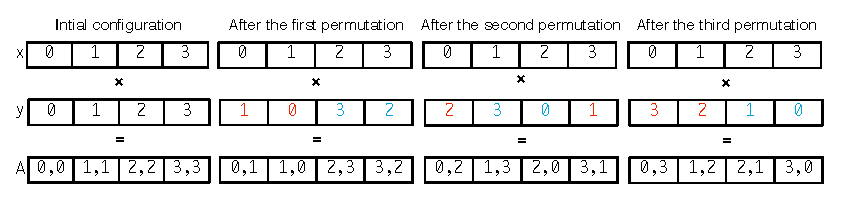
\includegraphics[scale=0.6]{lowlevelopt/pictures/vect-by-vect-inline.pdf}}
\caption{Outer-product vectorization by permuting values in a vector register.}
\label{fig:vect-by-vect}
\end{figure}

The storage layout of $A$, however, is incorrect after the application of this outer-product-based vectorization (\emph{op-vect}, in the following). It can be efficiently restored with a sequence of vector shuffles following the pattern highlighted in Figure~\ref{fig:restore-layout}, executed once outside of the \texttt{ijk} loop nest. The pseudo-code for the weighted Laplace assembly kernel using \emph{op-vect} is shown in Listing~\ref{code:weighted-laplace-opvect}.

\begin{figure}[h]
\centerline{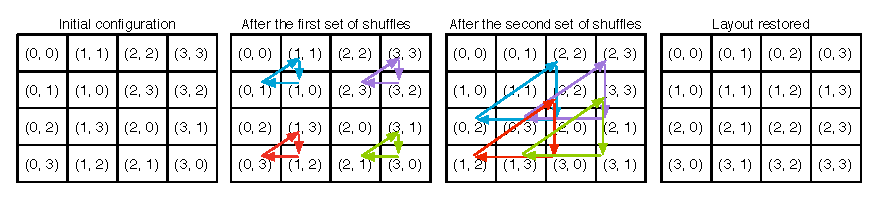
\includegraphics[scale=0.6]{lowlevelopt/pictures/vect-restore-inline.pdf}}
\caption{Restoring the storage layout after \emph{op-vect}. The figure shows how 4$\times$4 elements in the top-left block of the element matrix $A$ can be moved to their correct positions. Each rotation, represented by a group of three same-colored arrows, is implemented by a single shuffle intrinsic.}
\label{fig:restore-layout}
\end{figure}



\section{Experiments}
\label{sec:coffee-perfeval}

\subsection{Setup}
The objective is to evaluate the impact of the code transformations presented in the previous sections in three representative PDEs, which we refer to as (i) {\tt Helmholtz}, (ii) {\tt Diffusion}, and (iii) {\tt Burgers}. 

The three chosen equations are \emph{real-life kernels} and comprise the core differential operators in some of the most frequently encountered finite element problems in scientific computing. This is of crucial importance because distinct problems, possibly arising in completely different fields, may employ (subsets of) the same differential operators of our benchmarks, which implies similarities and redundant patterns in the generated code. Consequently, the proposed code transformations have a domain of applicability that goes far beyond that of the three analyzed equations.

The {\tt Helmholtz} and {\tt Diffusion} kernels are archetypal second order elliptic operators. They are complete and unsimplified examples of the operators used to model diffusion and viscosity in fluids, and for imposing pressure in compressible fluids. As such, they are both extensively used in climate and ocean modeling. Very similar operators, for which the same optimisations are expected to be equally effective, apply to elasticity problems, which are at the base of computational structural mechanics. The {\tt Burgers} kernel is a typical example of a first order hyperbolic conservation law, which occurs in real applications whenever a quantity is transported by a fluid (the momentum itself, in our case). We chose this particular kernel since it applies to a vector-valued quantity, while the elliptic operators apply to scalar quantities; this impacts the generated code, as explained next. The operators we have selected are characteristic of both the second and first order operators that dominate fluids and solids simulations.

The benchmarks were written in UFL (code available at~\citep{ufl-code-lowlevelopt}) and executed over real unstructured meshes through Firedrake. The {\tt Diffusion} code has already been shown in Listing~\ref{code:weighted-laplace}. The {\tt Helmholtz} equation uses the same differential operators as {\tt Diffusion}. In the {\tt Helmholtz} kernel code, the main differences with respect to {\tt Helmholtz} are the presence of additional arrays (the basis functions for the ``mass term'') and constants for computing the element matrix. {\tt Burgers} is a non-linear problem employing differential operators different from those of {\tt Helmholtz} and relying on vector-valued quantities, which has a major impact on the generated assembly code (see Listing~\ref{code:burgers}), where a larger number of basis function arrays ($X1$, $X2$, ...) and constants ($F0$, $F1$, ..., $K0$, $K1$,...) are generated.

These problems were studied varying both the shape of mesh elements and the polynomial order $q$ of the method, whereas the element family, Lagrange, is fixed. As might be expected, the larger the element shape and $q$, the larger the iteration space. Triangles, tetrahedra, and prisms were tested as element shape. For instance, in the case of {\tt Helmholtz} with $q=1$, the size of the \texttt{j} and \texttt{k} loops for the three element shapes is, respectively, $3$, $4$, and $6$. Moving to bigger shapes has the effect of increasing the number of basis function arrays, since, intuitively, the behaviour of the equation has to be approximated also along a third axis. On the other hand, the polynomial order affects only the problem size (the three loops \texttt{i}, \texttt{j}, and \texttt{k}, and, as a consequence, the size of $X$ and $Y$ arrays). A range of polynomial orders from $q=1$ to $q=4$ were tested; higher polynomial orders are excluded from the study because of current Firedrake limitations. In all these cases, the size of the element matrix rarely exceeds 30$\times$30, with a peak of 105$\times$105 in {\tt Burgers} with prisms and $q=4$.


\subsection{Impact of Transformations}

Experiments were run on a single core of an Intel architecture, a Sandy Bridge I7-2600 CPU running at 3.4 GHz, with 32KB of L1 cache and 256KB of L2 cache). The \texttt{icc 14.1}  compiler was used. On the Sandy Bridge, the compilation flags used were \texttt{-O2} and \texttt{-xAVX} for auto-vectorization (other optimization levels were tried, but they generally resulted in higher execution times).

\begin{figure}[t]
\centerline{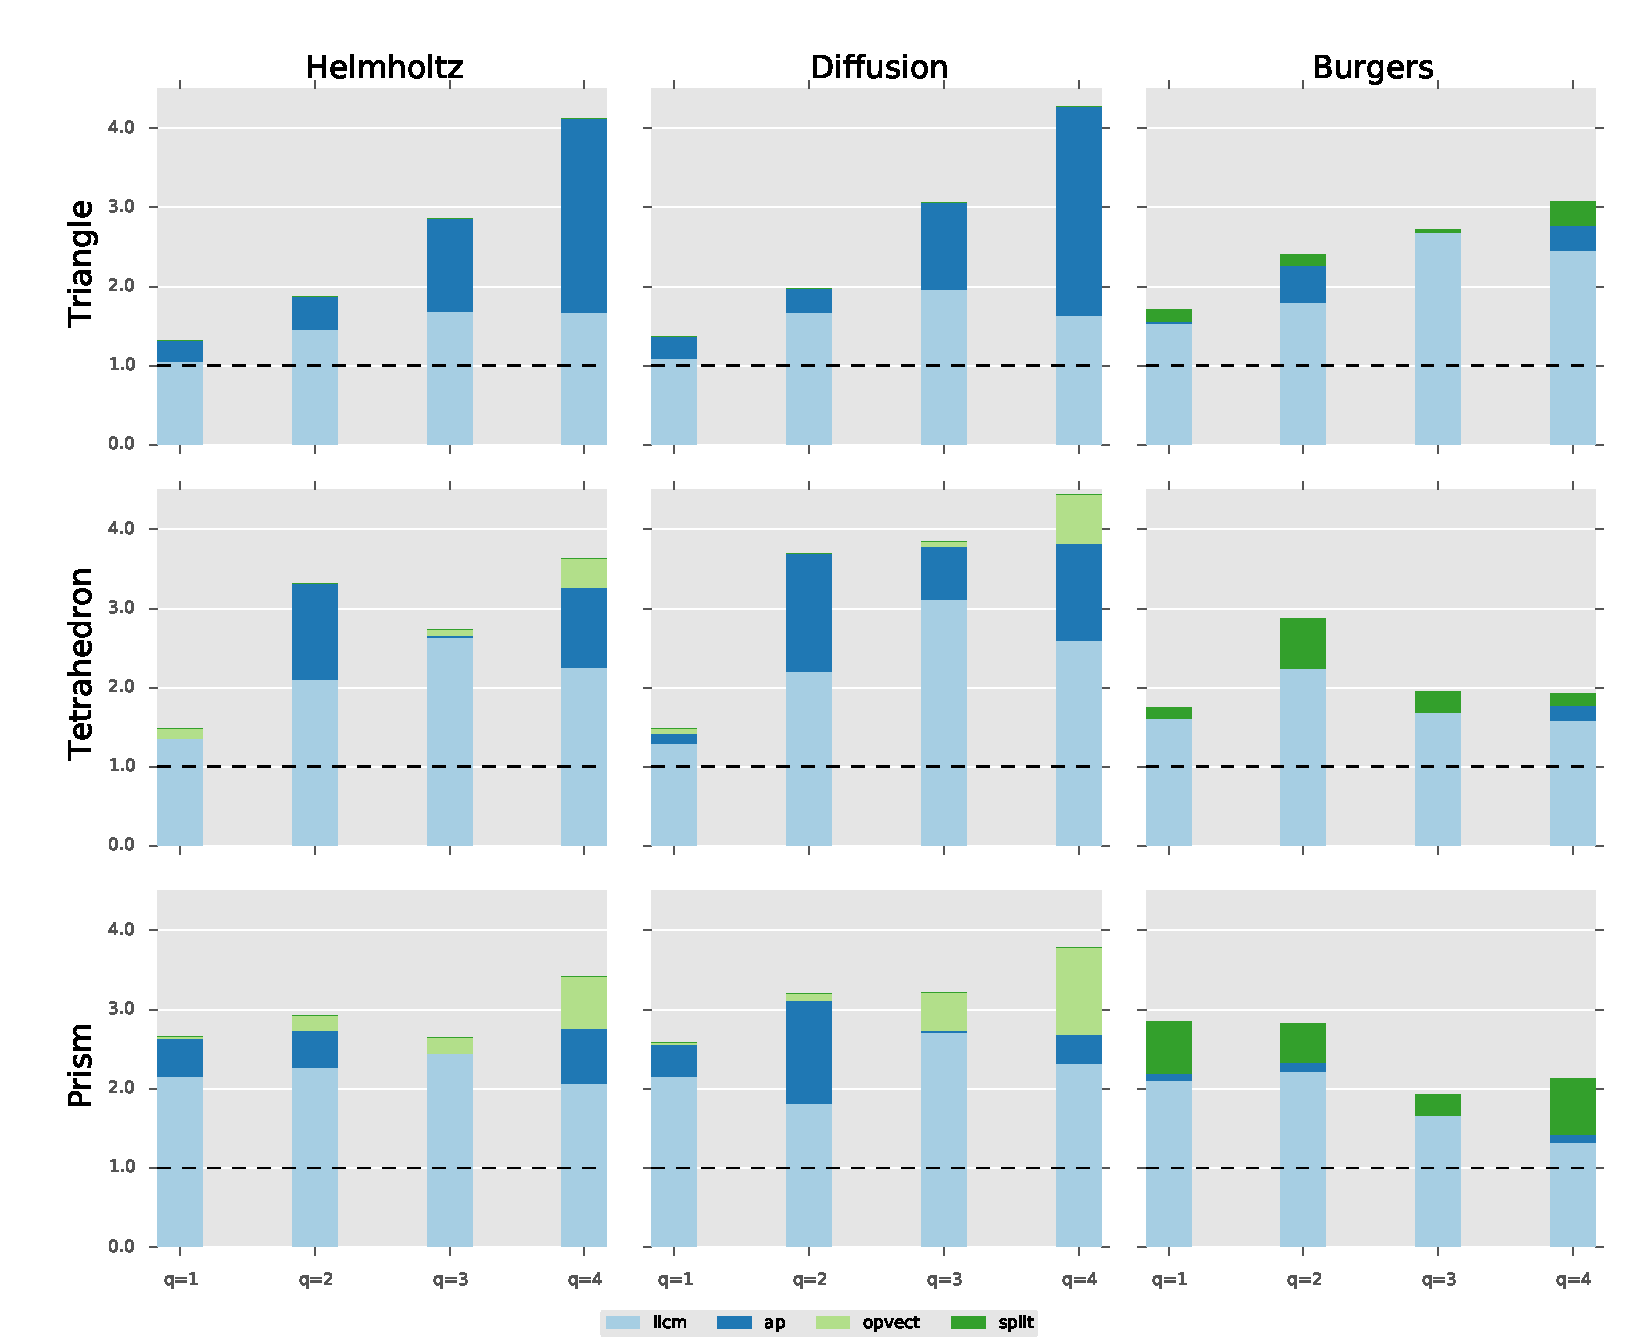
\includegraphics[scale=0.45]{lowlevelopt/perf-results/individual/plot_sb}}
\caption{Performance improvement due to generalized loop-invariant code motion (\emph{licm}), data alignment and padding (\emph{ap}), outer-product vectorization (\emph{op-vect}), and expression splitting (\emph{split}) over the original non-optimized code. In each plot, the horizontal axis reports speed ups, whereas the polynomial order $q$ of the method varies along the vertical axis.}
\label{fig:coffee-individual-res}
\end{figure}

The speed-ups achieved by applying the transformations on top of the original assembly kernel code are shown in Figure~\ref{fig:coffee-individual-res}. This figure is a three-dimensional plot: element shape and equation vary along the outermost axes, whereas $q$ varies within each sub-plot. In the next sections, we will refer to this figure and elaborate on the impact of the individual transformations. We shorten generalized loop-invariant code motion as \emph{licm}; padding and data alignment as \emph{ap}; outer-product vectorization as \emph{op-vect}; expression splitting as \emph{split}.

\subsubsection{Impact of Generalized Loop-invariant Code Motion}
\label{sec:perf-eval-licm}

In general, the speed-ups achieved by \emph{licm} are notable. The main reasons are that in the original code, (i) sub-expressions invariant to outer loops are not automatically hoisted, while (ii) sub-expressions invariant to the innermost loop are hoisted, but their execution is not auto-vectorized. These observations come from inspection of assembly code generated by the compiler.

The gain tends to grow with the computational cost of the kernels: bigger loop nests (i.e., larger element shapes and polynomial orders) usually benefit from the reduction in redundant computation, even though extra memory for the temporary arrays is required. Some discrepancies to this trend are due to a less effective auto-vectorization. For instance, on the Sandy Bridge, the improvement at $q=3$ is larger than that at $q=4$ because, in the latter case, the size of the innermost loop is not a multiple of the vector length, and a remainder scalar loop is introduced at compile time. Since the loop nest is small, the cost of executing the extra scalar iterations can have a significant impact.

\subsubsection{Impact of Padding and Data Alignment}
\label{sec:perf-eval-padding}

Padding, which avoids the introduction of a remainder loop as described in Section~\ref{sec:coffee-padding}, as well as data alignment, enhance the quality of auto-vectorization. Occasionally the impact of \emph{ap} is marginal. These may be due to two reasons: (i) the non-padded element matrix size is already a multiple of the vector length; (ii) the number of aligned temporaries introduced by \emph{licm} is so large to induce cache associativity conflicts (e.g. {\tt Burgers}).

\subsubsection{Impact of Vector-register Tiling}
\label{sec:perf-eval-opvect}

In this section, we evaluate the impact of vector-register tiling. \emph{op-vect} requires the unroll-and-jam factor to be explicitly set. Here, we report the best speed-up obtained after all feasible unroll-and-jam factors were tried. 

The rationale behind these results is that the effect of \emph{op-vect} is significant in problems in which the assembly loop nest is relatively big. When the loops are short, since the number of arrays accessed at every loop iteration is rather small (between 4 and 8 temporaries, plus the element matrix itself), there is no need for
vector-register tiling; extensive unrolling is sufficient to improve register re-use and, therefore, to maximize the performance. However, as the iteration space becomes larger, \emph{op-vect} leads to improvements up to 1.4$\times$ ({\tt Diffusion}, prismatic mesh, $q=4$ - increasing the overall speed up from 2.69$\times$ to 3.87$\times$).

Using the Intel Architecture Code Analyzer tool~\cite{IACA}, we confirmed that speed ups are a consequence of increased register re-use. In {\tt Helmholtz} $q=4$, for example, the tool showed that when using \emph{op-vect} the number of clock cycles to execute one iteration of the \texttt{j} loop decreases by roughly 17$\%$, and that this is a result of the relieved pressure on both of the data (cache) ports available in the core.

The performance of individual kernels in terms of floating-point operations per second was also measured. The theoretical peak on a single core, with the Intel Turbo Boost technology activated, is 30.4 GFlop/s. In the case of {\tt Diffusion} using a prismatic mesh and $q=4$, we achieved a maximum of 21.9 GFlop/s with \emph{op-vect} enabled, whereas 16.4 GFlop/s was obtained when only \emph{licm-ap} is used. This result is in line with the expectations: analysis of assembly code showed that, in the \texttt{jk} loop nest, which in this problem represents the bulk of the computation, 73$\%$ of instructions are actually floating-point operations.

Application of \emph{op-vect} to the {\tt Burgers} problem induces significant slowdowns due to the large number of temporary arrays that need to be tiled, which exceeds the available logical registers on the underlying architecture. Expression splitting can be used in combination with \emph{op-vect} to alleviate this issue; this is discussed in the next section.

%for which efficient register allocation can be already guaranteed

\subsubsection{Impact of Expression Splitting}
\label{sec:perf-results-split} 
Expression splitting relieves the register pressure when the element matrix evaluation needs to read from a large number of basis function arrays. As detailed in Section~\ref{sec:coffee-split}, the price to pay for this optimization is an increased number of accesses to the element matrix and, potentially, redundant computation. 

For the {\tt Helmholtz} and {\tt Diffusion} kernels, in which only between 4 and 8 temporaries are read at every loop iteration, \texttt{split} tends to slow down the computation, because of the aforementioned drawbacks. Slow downs up to 1.4$\times$ were observed. 

In the {\tt Burgers} kernels, between 12 and 24 temporaries are accessed at every loop iteration, so \emph{split} plays a key role since the number of available logical registers on the Sandy Bridge architecture is only 16. In almost all cases, a split factor of 1, meaning that the original expression was divided into two parts, ensured close-to-peak performance. The transformation negligibly affected register locality, so speed ups up to 1.5$\times$ were observed. For instance, when $q=4$ and a prismatic mesh is employed, the overall performance improvement increases from 1.44$\times$ to 2.11$\times$. 

The performance of the {\tt Burgers} kernel on a prismatic mesh was 20.0 GFlop/s from $q=1$ to $q=3$, while it was 21.3 GFlop/s in the case of $q=4$. These values are notably close to the peak performance of 30.4 GFlop/s. Disabling \emph{split} makes the performance drop to 17.0 GFlop/s for $q=1, 2$, 18.2 GFlop/s for $q=3$,
and 14.3 GFlop/s for $q=4$. These values are in line with the speed-ups shown in Figure~\ref{fig:coffee-individual-res}.

The \emph{split} transformation was also tried in combination with \emph{op-vect} (\emph{split-op-vect}). Despite improvements up to 1.22$\times$, \emph{split-op-vect} never outperforms \emph{split}. This is motivated by two factors: for small split factors, such as 1 and 2, the data space to be tiled is still too big, and register spilling affects run-time; for higher ones, sub-expressions become so small that, as explained in Section~\ref{sec:perf-eval-opvect}, extensive unrolling already allows to achieve a certain degree of register re-use.


\section{Experience with Traditional Compiler Optimizations}
\label{sec:coffee-genpurp-opts}

\subsection{Loop Interchange}
\label{sec:coffee-genpurp-opts-interchange}
All loops are interchangeable, provided that temporaries are introduced if the nest is not perfect. For the employed storage layout, the loop permutations \texttt{ijk} and \texttt{ikj} are likely to maximize the performance. Conceptually, this is motivated by the fact that if the \texttt{i} loop were in an inner position, then a significantly higher number of load instructions would be required at every iteration. We tested this hypothesis in manually crafted kernels. We found that the performance loss is greater than the gain due to the possibility of accumulating increments in a register, rather than memory, along the \texttt{i} loop. The choice between \texttt{ijk} and \texttt{ikj} depends on the number of load instructions that can be hoisted out of the innermost dimension. A good heuristics it to choose as outermost the loop along which the number of invariant loads is smaller so that more registers remain available to carry out the computation of the local element matrix. 

Our experience with the Intel's and GNU's compilers is controversial: if, from one hand, the former applies this transformation following a reasonable cost model, the latter results in general more conservative, even at highest optimization level. This behaviour was verified in different variational forms (by looking at assembly code and compiler reports), including the complex hyperelastic model analyzed in Chapter~\ref{ch:optimality}.

\subsection{Loop Unroll}
Loop unroll (or unroll-and-jam of outer loops) is fundamental to the exposure of instruction-level parallelism, and tuning unroll factors is particularly important.

We first observe that manual full (or extensive) unrolling is unlikely to be effective for two reasons. Firstly, the \texttt{ijk} loop nest would need to be small enough such that the unrolled instructions do not exceed the instruction cache, which is rarely the case: it is true that in a local assembly kernel the minimum size of the \texttt{ijk} loop nest is 3$\times$3$\times$3 (triangular mesh and polynomial order 1), but this increases rapidly with the polynomial order of the method and the discretization employed (e.g. tetrahedral meshes imply larger loop nests than triangular ones), so sizes greater than 10$\times$10$\times$10, for which extensive unrolling would already be harmful, are in practice very common. Secondly, manual unrolling is dangerous because it may compromise compiler auto-vectorization by either removing loops (most compilers search for vectorizable loops) or losing spatial locality within a vector register.

By comparison to implementations with manually-unrolled loops, we noticed that recent versions of compilers like GNU's and Intel's estimate close-to-optimal unroll factors when the loops are affine and their bounds are relatively small and known at compile-time, which is the case of our kernels. Our choice, therefore, is to leave the back-end compiler in charge of selecting unroll factors.

\subsection{Vector promotion}
\label{sec:coffee-precompute}
Vector promotion is a transformation that ``trades'' space in exchange of a parallel dimension (a ``clone'' of the integration loop), thus promoting SIMD vectorization at the level of an outer loop.

\begin{algorithm}
\scriptsize\ttfamily
\SetAlgorithmName{LISTING}{}

\KwSty{void} weighted$\_$laplace(\KwSty{double} A[3][3], \KwSty{double} **coords, \KwSty{double} w[3]) $\lbrace$\\
~~// Omitting redundant code \\
~~...\\
~~\KwSty{double} f0[3] = $\lbrace$0.0$\rbrace$;\\
~~\KwSty{for} (\KwSty{int} i = 0; i$<$6; i++) $\lbrace$ \\
~~~~\KwSty{for} (\KwSty{int} r  = 0; r < 3; ++r) $\lbrace$ \\
~~~~~~f0[i] += (w[r] * C[i][r]);\\
~~~~$\rbrace$ \\
~~$\rbrace$\\
~~\KwSty{for} (\KwSty{int} i = 0; i$<$6; i++) $\lbrace$ \\
~~~~\KwSty{double} T0[3] ALIGN;\\
~~~~\KwSty{double} T1[3] ALIGN;\\
~~~~\KwSty{for} (\KwSty{int} k = 0; k$<$3; r++) $\lbrace$ \\
~~~~~~T0[r] = ((K[1]*B[i][k])+(K[3]*D[i][k]));\\
~~~~~~T1[r] = ((K[0]*B[i][k])+(K[2]*D[i][k]));\\
~~~~$\rbrace$\\
~~~~\KwSty{for} (\KwSty{int} j = 0; j$<$3; j++) $\lbrace$\\
~~~~~~\KwSty{for} (\KwSty{int} k = 0; k$<$3; k++) $\lbrace$\\
~~~~~~~~A[j][k] += (T0[k]*T0[j] + T1[k]*T1[j])*det*W[i]*f0[i]);\\
~~~~~~$\rbrace$\\
~~~~$\rbrace$\\
~~$\rbrace$\\
$\rbrace$

\caption{The assembly kernel for the weighted Laplace operator in Listing~\ref{code:weighted-laplace} after application of vector promotion (on top of generalized code motion).}
\label{code:weighted-laplace-vector-prom}
\end{algorithm}

Consider Listing~\ref{code:weighted-laplace-vector-prom}. The evaluation of the coefficient \texttt{w} at each quadrature point can be vectorized by ``promoting'' \texttt{f} from a scalar to a vector of size 3. Any other sub-expression hoisted at the level of the integration loop (as described in Chapter~\ref{ch:optimality}) can be transformed in a similar way. The impact of this optimization obviously increases with the number of operations involving coefficients. At the same time, the allocation of extra memory may lead to the same issues described in Section~\ref{sec:mem-const}. Loop tiling could be used to counteract this negative effect, although this would significantly increase the implementation complexity.

We have not seen this transformation being applied by neither the GNU's nor the Intel's compilers. In our experience -- and in absence of loop tiling -- the impact on execution time is difficult to predict. This transformation requires further investigation. Despite being fully implemented in COFFEE, it is therefore not applied in the default optimization process.

\subsection{Loop Fusion}
\label{sec:coffee-loopfusion}
Loop fusion is a well-known compiler transformation that consists of merging a sequence of loops into a single one. This optimization can be applied by most general-purpose compilers. What we cannot expect these compilers to do, however, is identifying common sub-expressions across the fused loops -- an optimization of domain-specific nature.

In assembly kernels arising from bilinear forms, test and trial functions may belong to the same function space. More interestingly, the same operators could be applied to both sets of functions. This would result in both linear loops having the same iteration space and common sub-expressions arising across them. To avoid this kind of redundant computation and simultaneously enforcing fusion, we implemented in COFFEE a specialized version of loop fusion. In our experiments, this optimization always resulted in relatively small performance improvements, ranging between $2\%$ and $8\%$. Therefore, it is automatically enabled in the default optimization process.

\section{Related Work}
\label{sec:coffee-related-work}
The code transformations presented are inspired by standard compilers optimizations and exploit several domain properties. Our loop-invariant code motion technique individuates invariant sub-expressions and redundant computation by analyzing all loops in an iteration space, which is a generalization of the algorithms often implemented by general-purpose compilers. Expression splitting is an abstract variant of loop fission based on properties of arithmetic operators. The outer-product vectorization is an implementation of tiling at the level of vector registers; tiling, or ``loop blocking'', is commonly used to improve data locality (especially for caches). Padding has been used to achieve data alignment and to improve the effectiveness of vectorization. A standard reference for the compilation techniques re-adapted in this work is~\citep{dragonbook}.

Our compiler-based optimization approach is made possible by the top-level DSL, which enables automated code generation. DSLs have been proven successful in auto-generating optimized code for other domains: Spiral~\citep{Pueschel:05} for digital signal processing numerical algorithms, ~\citep{Spampinato:14} for dense linear algebra, or Pochoir~\citep{pochoir} and SDSL~\citep{stencil-compiler} for image processing and finite difference stencils. Similarly, PyOP2 is used by Firedrake to express iteration over unstructured meshes in scientific codes. COFFEE improves automated code generation in Firedrake.

Many code generators, like those based on the Polyhedral model~\citep{pluto} and those driven by domain-knowledge~\citep{modeldriven}, make use of cost models. The alternative of using auto-tuning to select the best implementation for a given problem on a certain platform has been adopted by nek5000~\citep{nek5000} for small matrix-matrix multiplies, the ATLAS library~\citep{ATLAS}, and FFTW~\citep{FFTW} for fast fourier transforms. In both cases, pruning the implementation space is fundamental to mitigate complexity and overhead. Likewise, COFFEE uses heuristics to steer the optimization process.


\section{Applicability to Other Domains}
\label{sec:generality}
We have demonstrated that our cross-loop optimizations for arithmetic intensity are effective in the context of automated code generation for finite element integration. In this section, we discuss their applicability in other computational domains and, in general, their integrability within a general-purpose compiler.

There are neither conceptual nor technical reasons which prevent our transformations from being used in other (general-purpose, research, ...) compilers. It is challenging, however, to assess the potential of the presented optimizations is another computational domains, and to what extent they would be helpful for improving the full application performance. To answer these questions, we first need to go back to the origins of our study. The starting point of our work was the mathematical formulation of a finite element operator, expressible as follows

\begin{equation}
\label{eq:assembly-model}
\scriptsize
\forall_{i, j} ~~~ A_{ij}^K = \sum_{q=1}^{n_1} \sum_{k=1}^{n_2} \alpha_{k, q}(a', b', c', ...) \beta_{q, i, j}(a, b, c, d, ...) \gamma_{q}(w_K, z_K)
\end{equation}

The expression represents the numerical evaluation of an integral at $n_1$ points in the mesh element $K$ computing the local element matrix $A$. Functions $\alpha$, $\beta$ and $\gamma$ are problem-specific and can be intricately complex, involving for example the evaluation of derivatives. We can however abstract from the inherent structure of $\alpha$, $\beta$ and $\gamma$ to highlight a number of aspects

\begin{itemize}
\item \textbf{Optimizing mathematical expressions.} Expression manipulation (e.g. simplification, decomposition into sub-expressions) opens multiple semantically equivalent code generation opportunities, characterized by different trade-offs in parallelism, redundant computation, and data locality. The basic idea is to exploit properties of arithmetic operators, such as associativity and commutativity, to re-schedule the computation suitably for the underlying architecture. Loop-invariant code motion and expression splitting follow this principle, so they can be re-adapted or extended to any domains involving numerical evaluation of complex mathematical expressions (e.g. electronic structure calculations in physics and quantum chemistry relying on tensor contractions, which we reviewed in Section~\ref{sec:bkg:tce}). In this context, we highlight three notable points.
\begin{enumerate}
\item In Equation~\eqref{eq:assembly-model}, the summations correspond to reduction loops, whereas loops over indices $i$ and $j$ are fully parallel. Throughout the paper we assumed that a kernel will be executed by a single thread, which is likely to be the best strategy for standard multi-core CPUs. On the other hand, we note that for certain architectures (for example GPUs) this could be prohibitive due to memory requirements. Intra-kernel parallelization is one possible solution: a domain-specific compiler could map mathematical quantifiers and operators to different parallelization schemes and generate distinct variants of multi-threaded kernel code. Based on our experience, we believe this is the right approach to achieve performance portability.
\item The various sub-expressions in $\beta$ only depend on (i.e. iterate along) a subset of the enclosing loops. In addition, some of these sub-expressions might reduce to the same values as iterating along certain iteration spaces. This code structure motivated the generalized loop-invariant code motion technique. The intuition is that whenever sub-expressions invariant with respect to different sets of affine loops can be identified, the question of whether, where and how to hoist them, while minimizing redundant computation, arises. Pre-computation of invariant terms also increases memory requirements due to the need for temporary arrays, so it is possible that for certain architectures the transformation could actually cause slowdowns (e.g. whenever the available per-core memory is small).
\item Associative arithmetic operators are the prerequisite for expression splitting. In essence, this transformation concerns resource-aware execution. In our context, expression splitting has successfully been applied to improve register pressure. However, the underlying idea of re-scheduling (re-associating) operations to optimize for some generic parameters is far more general. It could be used, for example, as a starting point to perform kernel fission; that is, splitting a kernel into multiple parts, each part characterized by less stringent memory requirements (a variant of this idea for non-affine loops in unstructured mesh applications has been adopted in~\citep{op2-lcpc}). In Equation~\eqref{eq:assembly-model}, for instance, not only can any of the functions $\alpha$, $\beta$ and $\gamma$ be split (assuming they include associative operators), but $\alpha$ could be completely extracted and evaluated in a separate kernel. This would reduce the working set size of each of the kernel functions, an option which is particularly attractive for many-core architectures in which the available per-core memory is much smaller than that in traditional CPUs.
\end{enumerate}
\item \textbf{Code generation and applicability of the transformations.} All array sizes and loop bounds, for example $n1$ and $n2$ in Equation~\ref{eq:assembly-model}, are known at code generation time. This means that ``good'' code can be generated. For example, loop bounds can be made explicit, arrays can be statically initialized, and pointer aliasing is easily avoidable. Further, all of these factors contribute to the applicability and the effectiveness of some of our code transformations. For instance, knowing loop bounds allows both generation of correct code when applying vector-register tiling and discovery of redundant computation  opportunities. Padding and data alignment are special cases, since they could be performed at run-time if some values were not known at code generation time. Theoretically, they could also be automated by a general-purpose compiler through profile-guided optimization, provided that some sort of data-flow analysis is performed to ensure that the extra loop iterations over the padded region do not affect the numerical results. 
\item \textbf{Multi-loop vectorization.} Compiler auto-vectorization has become increasingly effective in a variety of codes. However, to the best of our knowledge, multi-loop vectorization involving the loading and storing of data along a subset of the loops characterizing the iteration space (rather than just along the innermost loop), is not supported by available general-purpose and polyhedral compilers. The outer-product vectorization technique presented in this paper shows that two-loop vectorization can outperform standard auto-vectorization. In addition, we expect the performance gain to scale with the number of vectorized loops and the vector length (as demonstrated in  the Xeon Phi experiments). Although the automation of multi-loop vectorization in a general-purpose compiler is far from straightforward, especially if stencils are present, we believe that this could be more easily achieved in specific domains. The intuition is to map the memory access pattern onto vector registers, and then to exploit in-register shuffling to minimize the traffic between memory and processor. By demonstrating the effectiveness of multi-loop vectorization in a real scenario, our research represents an incentive for studying this technique in a broader and systematic way.
\end{itemize}

\section{Conclusions}
\label{sec:coffee-conclusion}
In this chapter, we have presented the study and systematic performance evaluation of a class of composable cross-loop optimizations for improving arithmetic intensity in finite element local assembly kernels. In the context of automated code generation for finite element local assembly, COFFEE is the first compiler capable of introducing low-level optimizations to simultaneously maximize register locality and SIMD vectorization. Assembly kernels have particular characteristics. Their iteration space is usually very small, with the size depending on aspects like the degree of accuracy one wants to reach (polynomial order of the method) and the mesh discretization employed. The data space, in terms of number of arrays and scalars required to evaluate the element matrix, grows proportionally with the complexity of the finite element problem. The various optimizations overcome limitations of current vendor and research compilers. The exploitation of domain knowledge allows some of them to be particularly effective, as demonstrated by our experiments on a state-of-the-art Intel platform. The generality and the applicability of the proposed code transformations to other domains has also been discussed.
